\chapter{Experiment and Result}
brief of experiment and result.
\section{Experiment}
Please tell how the experiment conducted from method.

\section{Result}
Please provide the result of experiment

\section{Cokro Edi Prawiro / 1164069}

\subsection{Teori}
\begin{enumerate}
\item Jelaskan apa itu klasifikasi teks, sertakan gambar ilustrasi buatan sendiri.\par
klasifikasi teks adalah cara untuk memilah-milah teks berdasarkan parameter tertentu baik itu jenis teks atau jenis dari dokumen yang terdapat kumpulan teks didalamnya, sedangkan teks itu sndiri merupakan sekumpulan kata yang dapat dibaca. bisa berupa buku, majalah, rambu-rambu dan lain sebagainya. agar lebih jelas dapat dilihat pada gambar \ref{c55}

\item Jelaskan mengapa klasifikasi bunga tidak bisa menggunakan machine learning, sertakan ilustrasi sendiri.\par
Klasifikasi bunga tidakdapat menggunakan mesin learning dikarenakan jenis-jenis bunga banyak yang mirip bahkan banyak bunga yang serupa tetapi tidak sama. oleh karena itu klasifikasi bunga tidakbisa di gunakan oleh mesin learning dikarenakan jika salah satu inputan ciri-ciri dari siatu bunga di inputkan kemungkinan jawaban dari mesin learning itu tidak tepat contoh dimasukan inputan ciri ciri bunga mawar putih kemudian mesin learning menjawab bahwa itu bunga mawar merah. untuk lebih jelasnya dapat dilihat pada gambar \ref{c56}

\item Jelaskan bagaimana teknik pembelajaran mesin pada teks pada kata-kata yang digunakan di youtube,jelaskan arti per atribut data csv dan sertakan ilustrasi buatan sendiri.\par
cara pembelajaran teks yang di gunakan youtube yaitu dengan cara merekam data yang sering di inputkan oleh user pada menu pencarian youtube. sehingga pada saat user akan mencari data yang serupa seringkali youtube menyediakan opsi atau rekomendasi-rekomendasi dari pencaharian. contoh saya menuliskan m maka muncul opsi pilihan master chep dan lainya yang berawalan m rekomendasi yang muncul merupakan kata-kata yang sering di cari oleh banyak user atau sering di buka oleh user itu sendiri untuk lebih jelasnya dapat dilihat pada gambar \ref{c57}

\item Jelaskan apa yang dimaksud vektorisasi data.\par
vektorisasi data merupakan pemechan data menjadi bagian bagian yang lebih sederhana contoh pada satu paragraf terdiri dari 200 kata kemudian dilakukan vektorisasi dengancara membagi-bagi kata dalam paragraf tersebut ke dalam kalimat-kalimat yang terpisah kemudian di pecah lagi menjadi data dalam perkata selanjutnya kata kata tersebut di terjemahkan.

\item Jelaskan apa itu bag of words dengan kata-kata yang sederhana dan ilustrasi sendiri.
 bag of words merupakan peroses penyederhanaan kata-kata yang asalnya tersiri dalam satu kalimat atau satu paragraf di ubah menjadi perkata kemudian kata-kata tersebut di kumpulkan menjadi satu kelompok tanpa ada arti dari kata-kata yang telah di kumpulkan tersebut lalu di hitung frekuensi kemunculan dari kata tersebut. supaya lebih jelas dapat dilihat pada contoh gambar \ref{c58} :

\item Jelaskan apa itu TF-IDF, ilustrasikan dengan gambar sendiri.
 TF-IDF merupakan metode untuk menghitung bobot dari kata yang sering muncul pada suatu kalimat. metode ini menghitung nilai TF atau Term Frequency dan IDF atau Inverse Document Frequency pada setiap kata pada kalimat yang dijadikan acuan kata pada metode ini sering di sebut token adapun rumus dari metode ini dapat dilihat pada gambar \ref{c59} dan untuk hasil ujicobanya dapat di lihat pada gambar \ref{c60} dan gambar \ref{c61}.

\end{enumerate}

\subsection{Praktek Program}

\subsection{Penanganan Error}

\begin{figure}
      \centerline{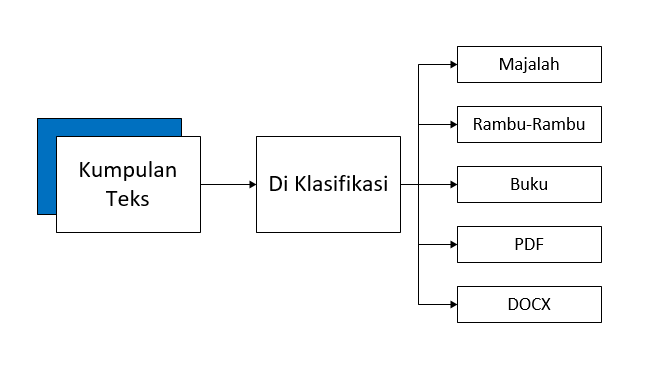
\includegraphics[width=1\textwidth]
      {figures/cokro/c55}}
      \caption{Ilustrasi clasifikasi Teks}
      \label{c55}
      \end{figure}

\begin{figure}
      \centerline{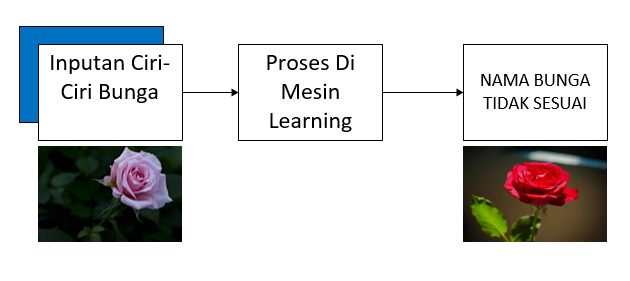
\includegraphics[width=1\textwidth]
      {figures/cokro/c56}}
      \caption{Ilustrasi Bunga Tidak bisa dibaca di Mesin Learning}
      \label{c56}
      \end{figure}

\begin{figure}
      \centerline{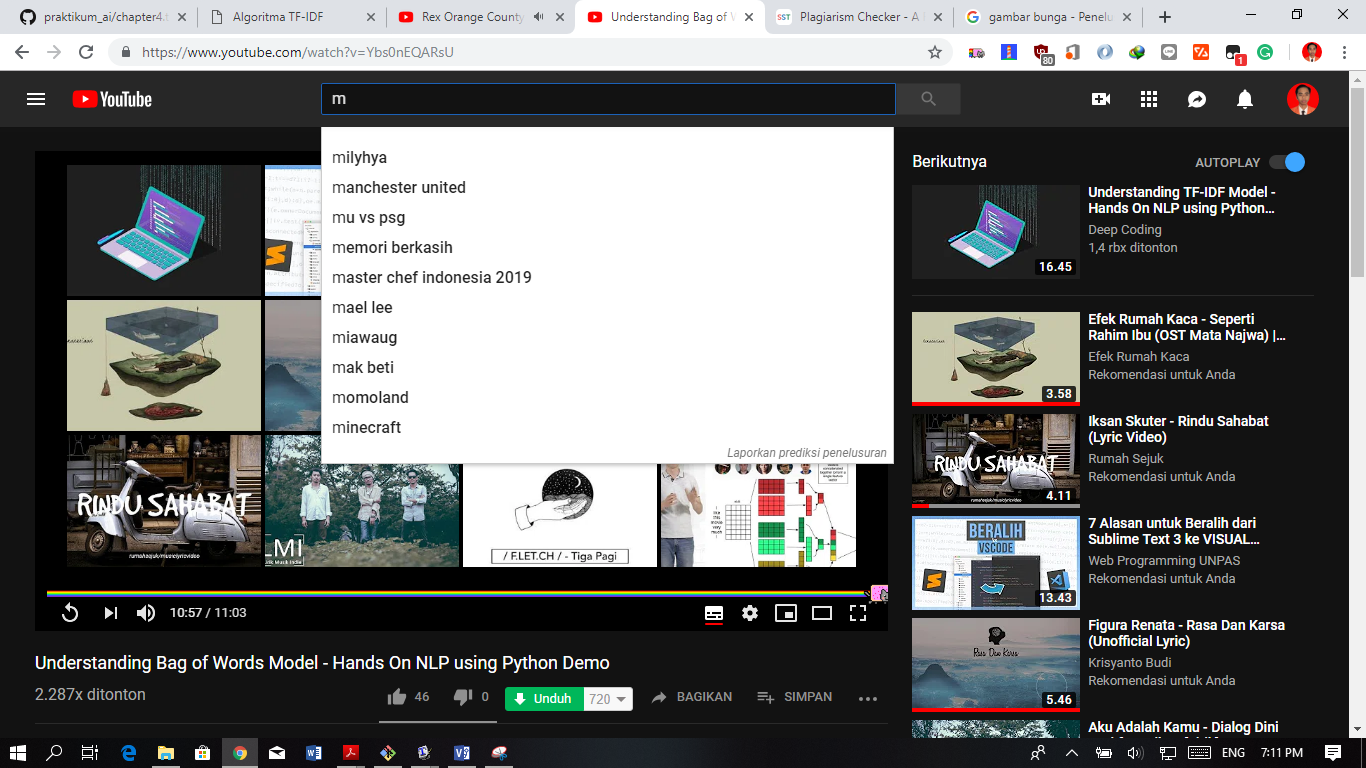
\includegraphics[width=1\textwidth]
      {figures/cokro/c57}}
      \caption{contoh hasil pembelajaran text di youtube}
      \label{c57}
      \end{figure}

\begin{figure}
      \centerline{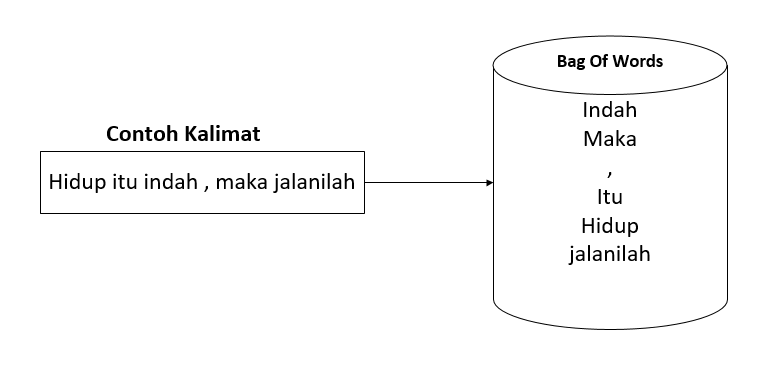
\includegraphics[width=1\textwidth]
      {figures/cokro/c58}}
      \caption{Ilustrasi bag of words}
      \label{c58}
      \end{figure}

\begin{figure}
      \centerline{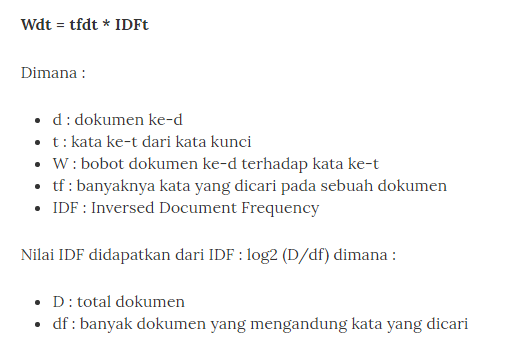
\includegraphics[width=1\textwidth]
      {figures/cokro/c59}}
      \caption{Rumus  TF-IDF}
      \label{c59}
      \end{figure}

\begin{figure}
      \centerline{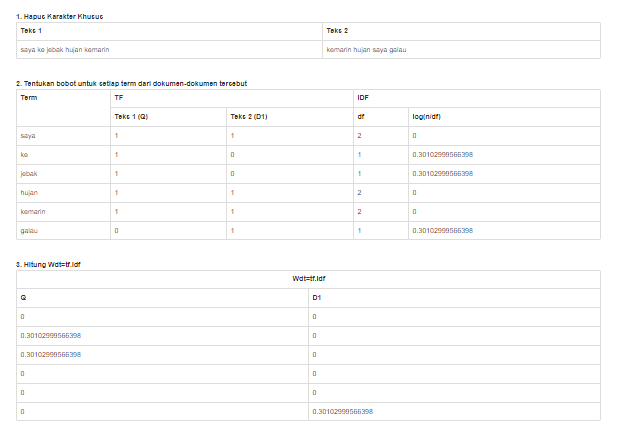
\includegraphics[width=1\textwidth]
      {figures/cokro/c60}}
      \caption{Hasil Perhitungan TF-IDF}
      \label{c60}
      \end{figure}

\begin{figure}
      \centerline{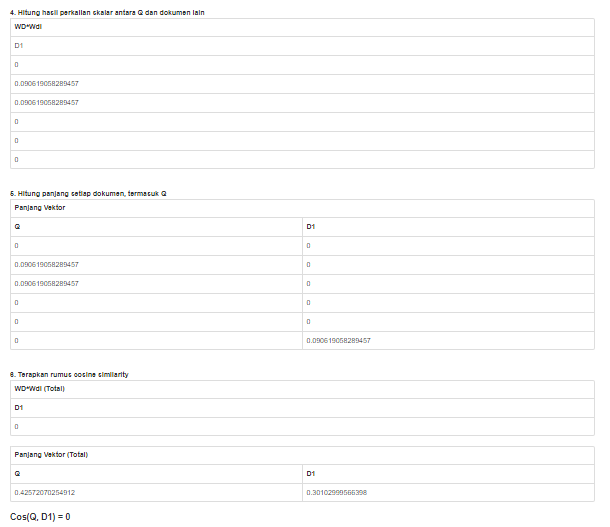
\includegraphics[width=1\textwidth]
      {figures/cokro/c61}}
      \caption{Hasil Perhitungan  TF-IDF}
      \label{c61}
      \end{figure}

\section{Fathi Rabbani / 1164074}
\subsection{Teori}
\begin{enumerate}
\item Klasifikasi Teks
\subitem klasifikasi teks adalah sebuah cara dalam memilah data teks berdasarkan beberapa parameter tertentu dengan data yang bersifat dokumen ataupun teks yang memiliki kumpulan - kumpulan teks didalamnya, serta teks itu sendiri merupakan sebuah data yang bisa dibaca oleh manusia atau bisa disebut juga dengan tipe data karakter atau string yang mudah untuk diolah seperti pada buku, majalah, koran, jurnal dan lainya. untuk ilustrasi dari klasifikasi teks bisa dilihat pada gambar \ref{coba1}
\begin{figure}[!htbp]
	\centering
	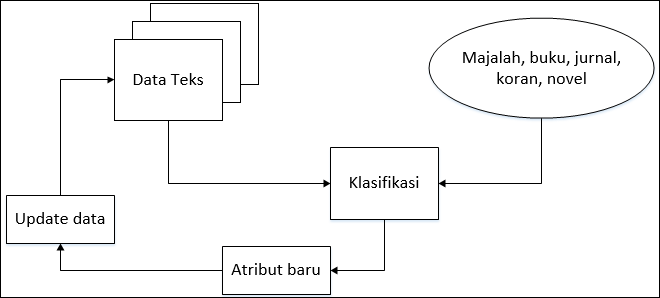
\includegraphics[width=1\textwidth]{figures/fathi/chapter4/hari1/1}
	\caption{Klasifikasi Teks}
	\label{coba1}
\end{figure}

\item Mengapa Klasifikasi Bunga tidak dapat menggunakan Machine Learning
\subitem klasifikasi menggunakan tipe data yang dimana attributenya memiliki nilai data berupa vektor dengan perbandingan masing - masing data yang dimiliki memiliki sedikit perbedaan, sehingga program atau sistem tidak dapat membedakan dengan tepat antara gambar 1 dan gambar 2 dikarenakan memiliki perbedaan yang hampir tidak dapat dilihat pada beberapa contoh gambar. untuk ilustrasi dapat dilihat pada gambar \ref{coba2}
\begin{figure}[!htbp]
	\centering
	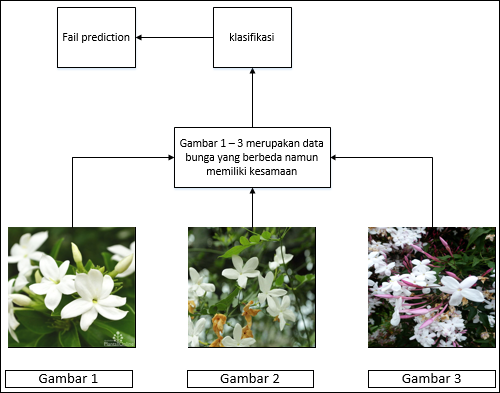
\includegraphics[width=1\textwidth]{figures/fathi/chapter4/hari1/2}
	\caption{Klasifikasi Bunga}
	\label{coba2}
\end{figure}

\item Teknik Pembelajaran Youtube pada Teks
\subitem Youtube merupakan platform untuk berbagi pengalaman video para penggunanya, dan yotube menggunakan machine learning dengan membaca data yang penggunanya inputkan disebut juga temporary data, yang menyimpan data pencarian para penggunanya dengan membuatkan kolom klasifikasinya seperti pada gambar \ref{coba3}, dimana data pencarian saya memliki 6 data dengan jumlah atribut yang masuk adalah 15.
\begin{figure}[!htbp]
	\centering
	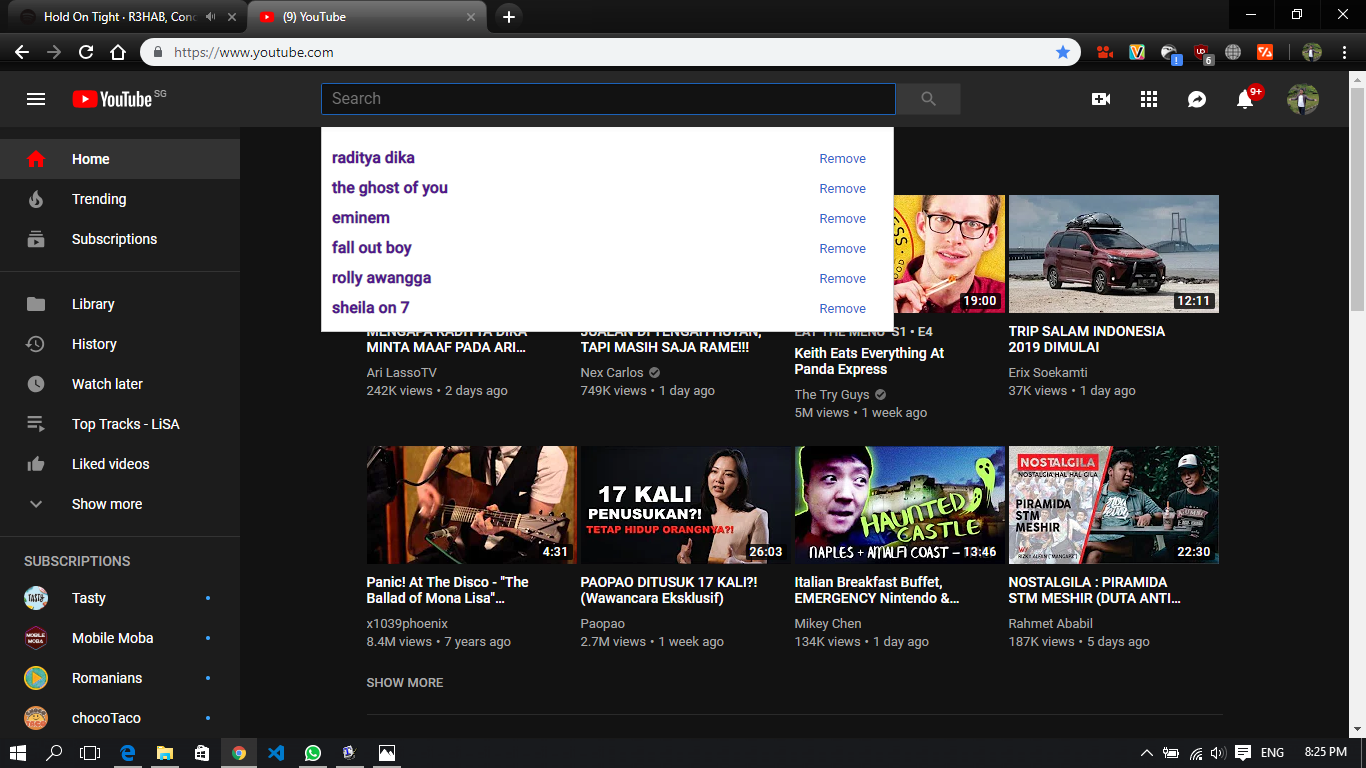
\includegraphics[width=1\textwidth]{figures/fathi/chapter4/hari1/3}
	\caption{Data Youtube}
	\label{coba3}
\end{figure}

\item Vektorisasi Data
\subitem vektor adalah tipe data yang digunakan untuk mempelajari data gambar agar mudah untuk diproses serta lebih sederhana dalam hasil yang dikeluarkan, dan data yang telah divektorisasi terpecah - pecah menjadi beberapa atribut agar mudah untuk diproses.

\item Bag of Words
\subitem kumpulan data teks yang diproses dan dibuatkan atribut barunya jika data yang dimiliki sudah tersedia, pada gambar \ref{coba4}, menjelaskan jika data yang sama tidak akan diproses menjadi atribut baru sehingga data tersebut sudah disimpan dan akan memproses data baru yang belum dimiliki.
\begin{figure}[!htbp]
	\centering
	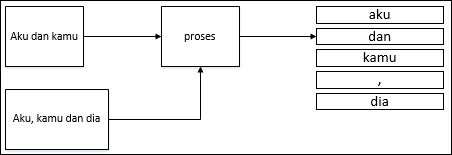
\includegraphics[width=1\textwidth]{figures/fathi/chapter4/hari1/4}
	\caption{Bags of Word}
	\label{coba4}
\end{figure}

\item TF-IDF
\subitem merupakan sebuah metode dalam sebuah perhitungan untuk menghitung bobot dari setiap kata - kata yang sering muncul dalam sebuah kalimat. metode ini sendiri menghitung data nilai dari TF(term of frequency) dan data IDF(inverse document frequency) yang dijadikan sebagai data yang dapat diproses, seperti berikut ini :
\begin{itemize}
\item proses pertama adalah dengan membuat data yang akan diolah seperti pada data 
\begin{verbatim}
–  gold
–  silver
–  truck

Untuk koleksi dokumennya terdapat:

dokumen 1 (d1) = Shipment of gold damaged in a fire
dokumen 2 (d2) = Delivery of silver arrived in a silver truck
dokumen 3 (d3) = Shipment of gold arrived in a truck

Jadi total jumlah dokumen adalah koleksi dokumen (D) = 3
\end{verbatim}

\item proses kedua adalah menggabungkan ke 3 data tersebut dengan menghilangkan nilai yang di ulang (term of frequency)-nya dan hasilnya adalah seperti pada 
\begin{verbatim}
– ship – gold – damage – fire – deliver – silver – arrive – truck
\end{verbatim}

\item kedua proses tersebut dinamakan preprocessing text, dan berikut ini adalah formula yang digunakan untuk menghitung nilai pada bobot data d2 pada
\begin{verbatim}
Wij = TFij x log(D/DFj) + 1
Wij = 2 x (log(3/1) + 1)
Wij = 2 x (0.477 + 1)
Wij = 2.954
\end{verbatim}

\item dengan nilai yang dimiliki seperti itu maka untuk hasilnya adalah seperti pada gambar \ref{coba5}
\begin{figure}[!htbp]
	\centering
	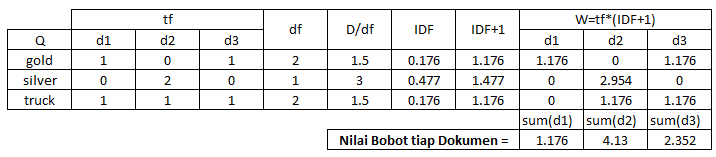
\includegraphics[width=1\textwidth]{figures/fathi/chapter4/hari1/5}
	\caption{TF-IDF}
	\label{coba5}
\end{figure}
\end{itemize}
\end{enumerate}